\documentclass[a4paper]{article}
\usepackage[ngerman]{babel}
\usepackage[T1]{fontenc}
\usepackage[utf8]{inputenc}
\usepackage{textcomp}
\usepackage{geometry}
\geometry{ left=2cm, right=2cm, top=2cm, bottom=4cm, bindingoffset=5mm}
\usepackage{graphicx}
\usepackage{xcolor}
\usepackage{hyperref}
\date{}
\author{}
\usepackage{fancyhdr}
\pagestyle{fancy}
\fancyhf{}
\fancyhead[R]{3141241 - Jamie Ullerich \\ 2892258 - Gerhard Breul \\ 2973140 - Felix Bühler}
\fancyhead[L]{Information Visualisation and Visual Analytics \\ WS 2019/20 }
\renewcommand{\headrulewidth}{0.5pt}
\usepackage{tikz}
\usetikzlibrary{calc}
\usepackage{amsmath}



\title{\textbf{Assignment 4}}

\begin{document}
\maketitle 
\thispagestyle{fancy}

\section*{Task 1 - Graph Representation}
\begin{enumerate}
	\item[a)]
	Since the given data contains only European countries, we decided to use a map, as this facilitates finding the desired country at a glance. 
	The preferred holiday destinations are drawn as edges between the countries, where the thickness corresponds to the percentage of the survey. 
	To avoid visual clutter, we suggest to use edge bundling. 
	It is possible to add arrowheads to include the direction. 
	The sketched visualisation below does not show the exact values of the given data since it would be rather complicated to calculate this by hand. 
	%(see task d) for exact data) 
	
	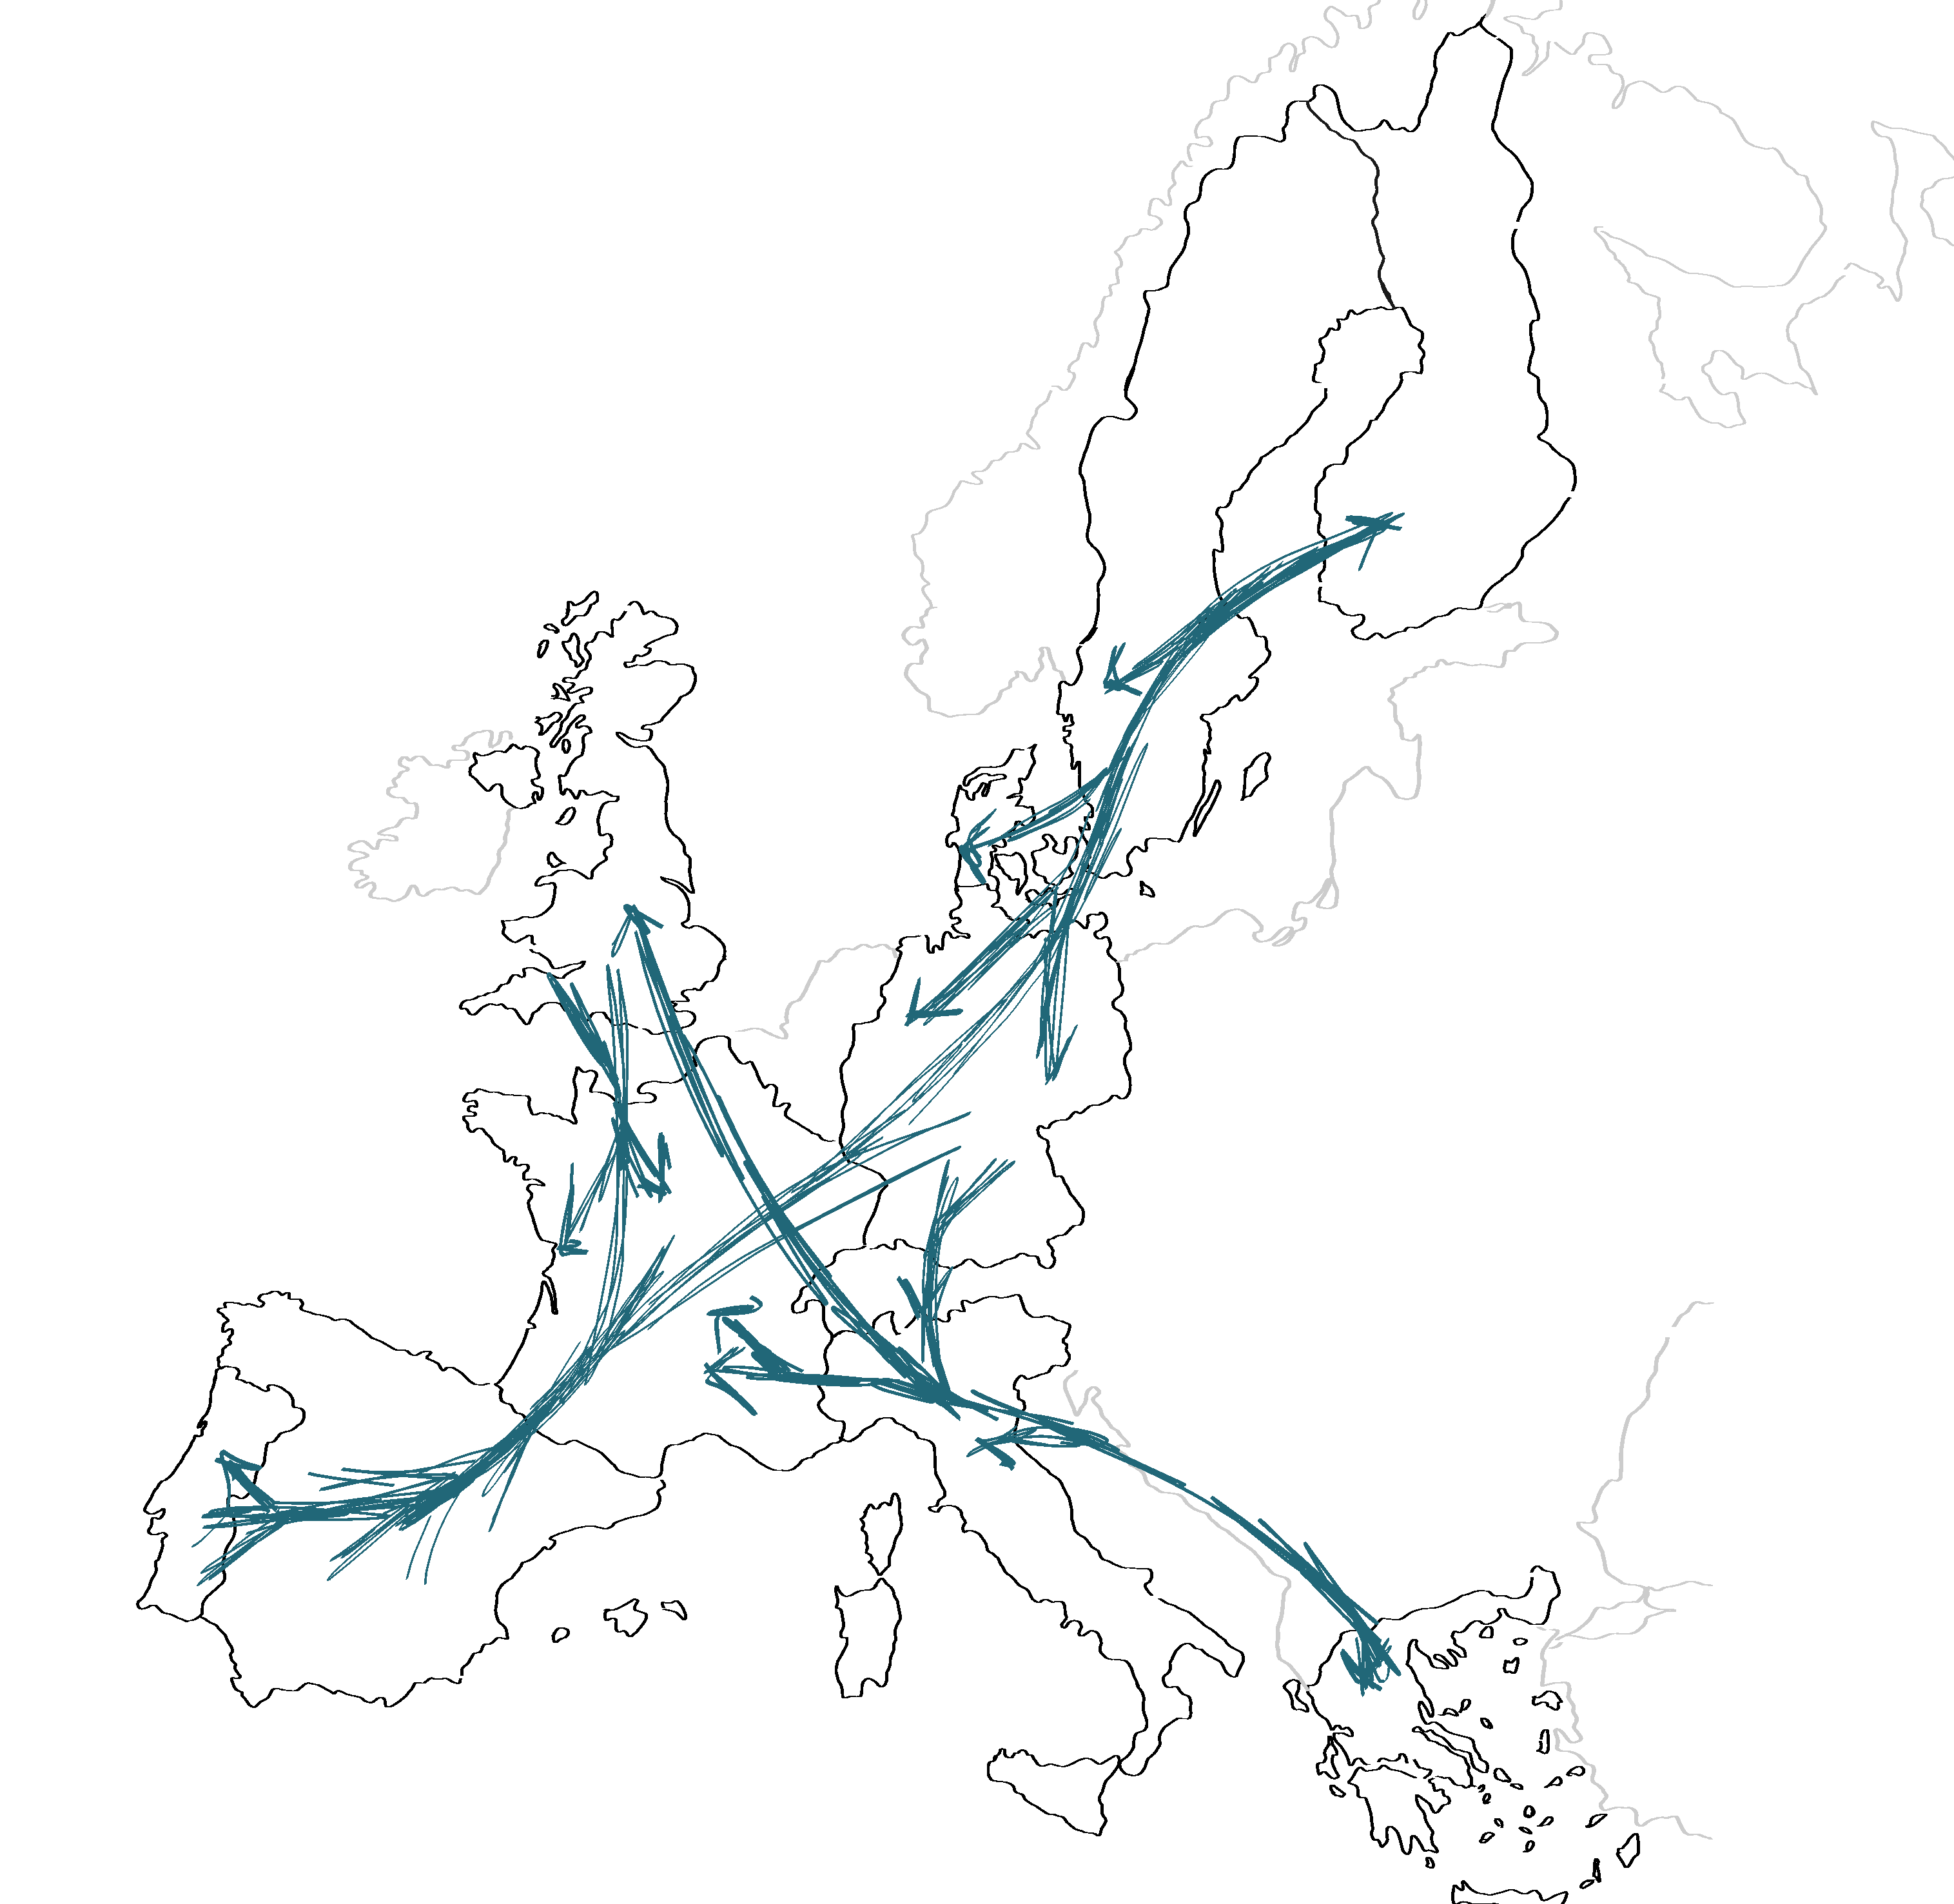
\includegraphics[width=\linewidth]{task1_a.pdf}
	\newpage
	\item[b)]
	In our extended visualisation, the border thickness of the countries corresponds to the population and the colour represents the average temperature. 
	
	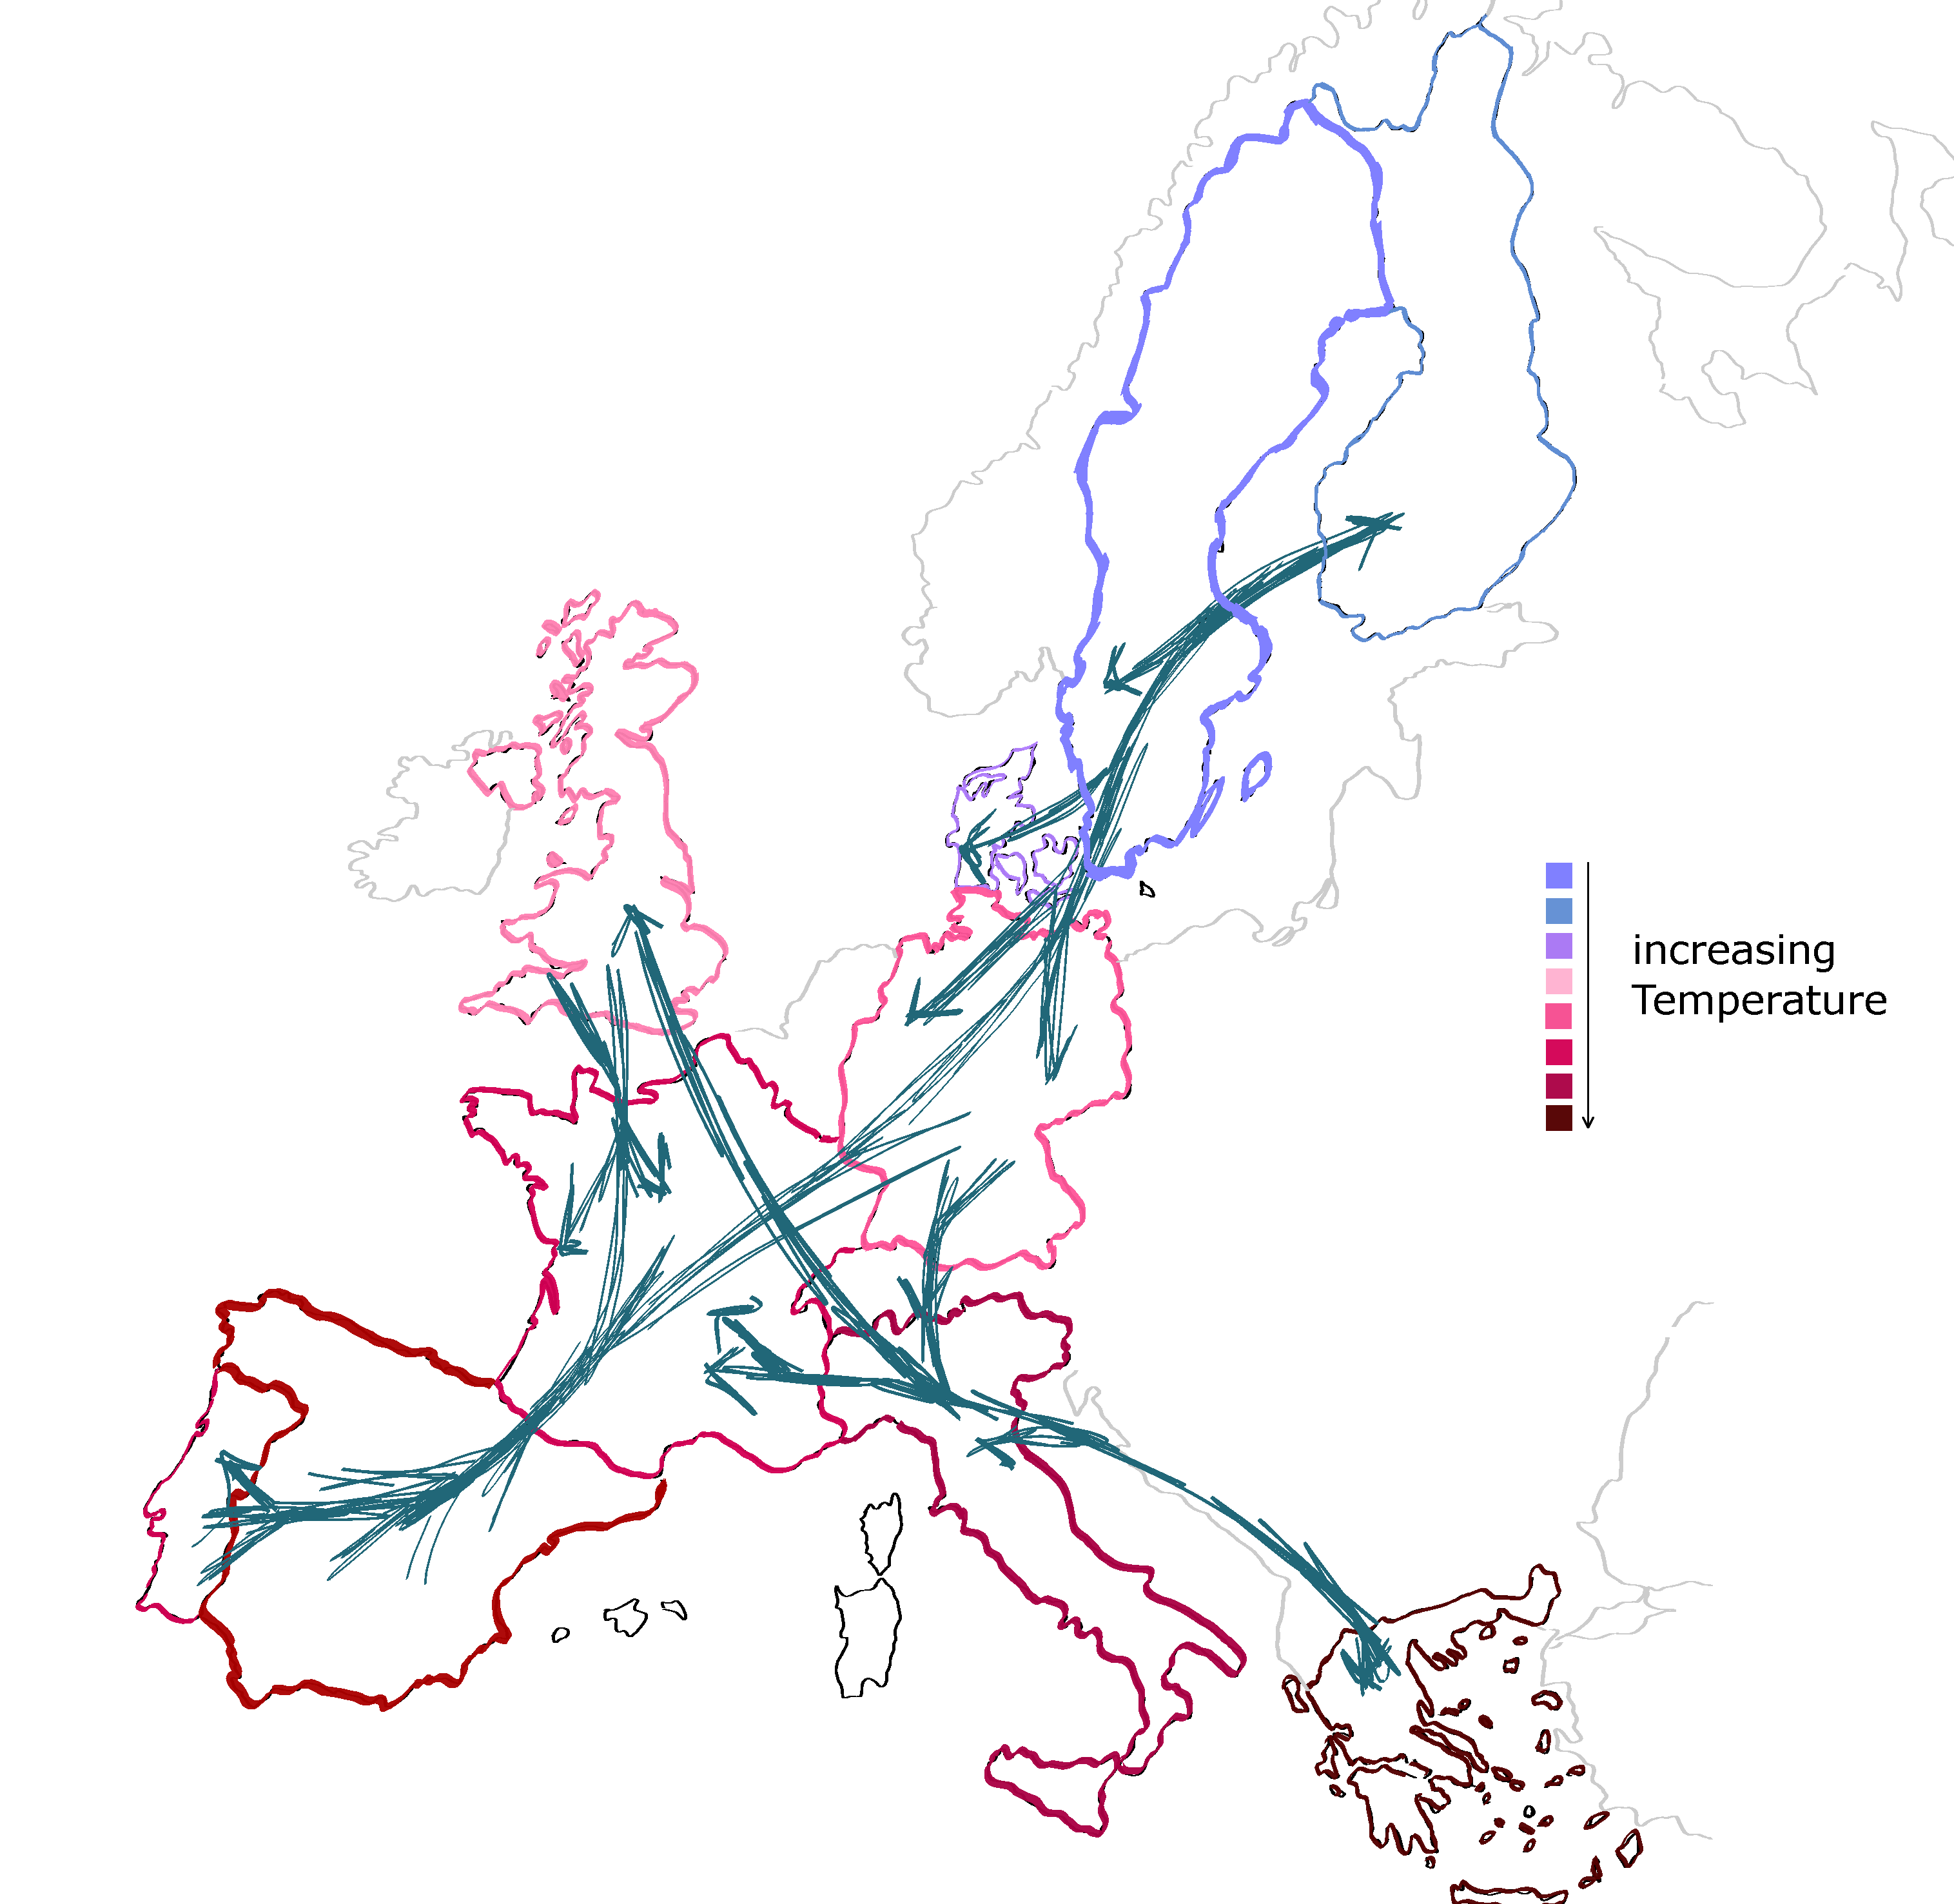
\includegraphics[width=\linewidth]{task1_b.pdf}
	
	\item[c)] 
	In our visualisation from task a), it is easier to find the countries since the map is more descriptive than simple country codes. 
	Additionally, the arrows are easier to understand. 
	A drawback of the edge bundling visualisation in comparison with the matrix visualisation is, that it is only possible to see which countries are connected, but the exact data cannot be read of the map. 
	Besides the data about the destinations, the percentage of people from the survey is also easier to see in the matrix. 
	
	Both techniques are suited for this task. 
	It might be better to choose the map for applications where exact data is not needed like a newspaper article, where the focus is on a fast and clear overview. 
	The matrix visualisation can be used for a more scientific application like the presentation of the survey, since it is more important to have the exact data here (meaning that there are still no numbers but the percentage can be estimated easier). 
	
\end{enumerate}

\section*{Task 2 - Force-directed Graph Layouts}
\begin{enumerate}
	\item[a)]
	The initial layout after 0 iterations: \\
	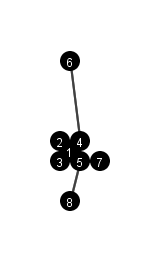
\includegraphics{0.png}
	
	\item[b)]
	The layout after 1, 5, 10, 25, 50, and 100 iterations:\\
	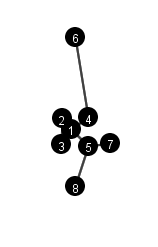
\includegraphics{1.png}
	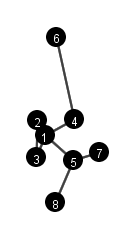
\includegraphics{5.png}
	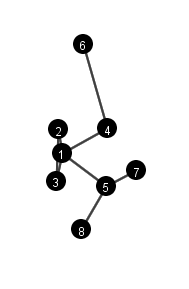
\includegraphics{10.png}\\
	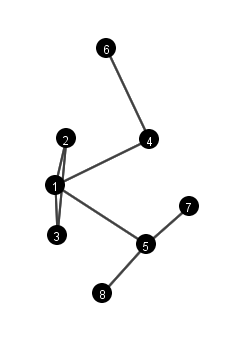
\includegraphics{25.png}\\
	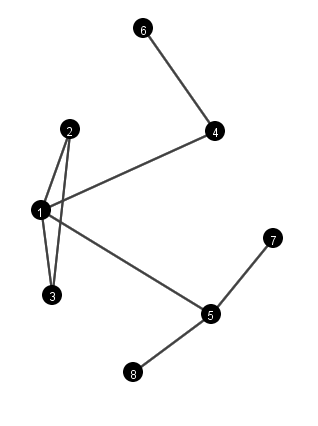
\includegraphics{50.png}\\
	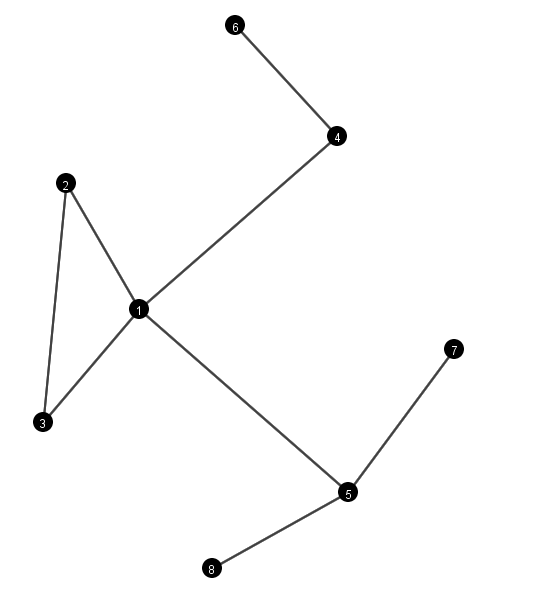
\includegraphics{100.png}
	\newpage
	\item[c)]The final graph\\
	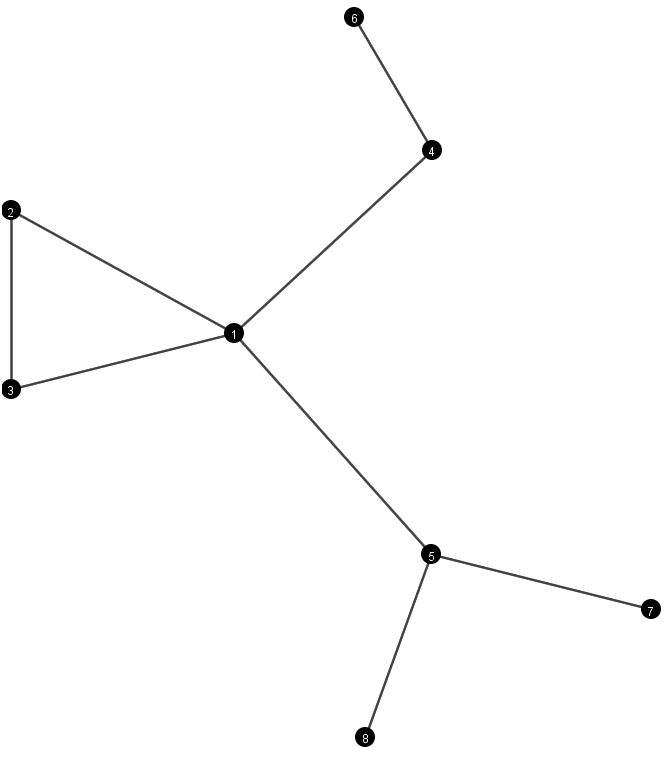
\includegraphics[width=15cm]{350+.png}
		
\end{enumerate}
\end{document}
